\documentclass[a4paper,dvipdfmx]{jarticle}
% 数式用
\usepackage{amsmath, amsfonts}  % 数式用
\usepackage{bm} % 数式中の太字
\usepackage{amssymb} % 記号
% 画像用
\usepackage{float} % 画像の挿入箇所を固定
\usepackage[dvipdfmx]{graphicx} % 画像挿入用
\usepackage{wrapfig} % 画像の周りに本文を流し込み
% ページレイアウト
\usepackage{here} % 画像を強制的に出力
\usepackage{url} % URLリンク
\usepackage{hyperref} % 
\hypersetup{
  colorlinks=false, % リンクに色をつけない設定
  bookmarks=true, % 以下ブックマークに関する設定
  bookmarksnumbered=true, % ブックマークに節番号などをつけるか
  pdfborder={0 0 0}, % 枠なし
  bookmarkstype=toc % 目次情報のブックマークを作る
}
\usepackage[margin=20truemm]{geometry} %余白調整
% 文字装飾
\usepackage{color}
\usepackage{ascmac}
\usepackage{fancybox}
\begin{document}
\begin{titlepage}
  \centering
  \LARGE
  外部設計書
  \\\vspace{1cm}
  地域密着型アルバイト求人アプリ\\
  \textbf{REEL(Region Event Excitement Linkup)}
  \\\vspace{4cm}
  第 1.0 版
  \\\vspace{4cm}
  \today
  \\\vspace{2.5cm}
  \textbf{ChaO!株式会社}
\end{titlepage}
\tableofcontents
\newpage
\section{はじめに}
本書では、弊社がシステム提案書で提案した地域密着型アルバイト求人アプリ「REEL」の詳細について示す。
まず、本システムの要件を整理する。
なお、主張の根拠はシステム提案書を参照されたい。
その後、主に機能要件に関わる機能設計・UI設計を説明する。
そして最後に、主に非機能要件に関わるデータベース設計・ネットワーク設計・運用・保守を説明する。

\section{システム概要}
本アプリケーションREELは、イベント主催者や地域の法人などがイベント告知や、求人の掲載をスマートフォン上で行うことができるアプリケーションである。また、一般利用者はそれらの掲載された情報を基に、イベントや求人を検索することができる。本アプリケーションは、イベントや求人の掲載を行うことで、地域の活性化を図ることを目的としている。
それぞれのユーザーは初めに利用規約に同意し、ユーザー登録を行うことで本アプリケーションを利用することができる。
\section{機能設計}

\subsubsection{一般利用者}

\subsubsection{法人利用者}

\section{UI設計}

\subsubsection{一般利用者}

\subsubsection{法人利用者}

\section{運用保守設計}

\section{データベース設計}

\section{ネットワーク設計}
サーバコンピュータとして、Amazon Web Servicesを用いる。以下に使用するサービスを記述する。
\begin{table}[H]
  \centering
  \caption{使用するサービス}
  \label{tab:services}
  \begin{tabular}{|c|c|} \hline
    サービス名                            & 用途            \\ \hline \hline
    Amazon Elastic Container Service & コンテナの実行環境     \\ \hline
    Amazon App Runner                & デプロイ          \\ \hline
    Amazon RDS                       & データベース        \\ \hline
    Amazon S3                        & データベースのバックアップ \\ \hline
    Amazon Route 53                  & ドメイン名の取得      \\ \hline
  \end{tabular}
\end{table}
また、使用するソフトウェアやフレームワークを以下に記述する。
\begin{table}[H]
  \centering
  \caption{使用するソフトウェア・フレームワーク}
  \label{tab:software}
  \begin{tabular}{|c|c|} \hline
    ソフトウェア・フレームワーク名 & 用途         \\ \hline \hline
    Docker          & コンテナ型仮想化技術 \\ \hline
    MySQL           & データベース     \\ \hline
    FastAPI         & RestAPIの実装 \\ \hline
    Flutter         & フロントエンドの実装 \\ \hline
  \end{tabular}
\end{table}

図\ref{fig:network-design}は、本アプリにおけるネットワークの構成を示している。
ユーザーは、Flutterで実装されたフロントエンドから、FastAPIで実装されたバックエンドに対して、HTTPリクエストを送信する。
バックエンドは、Amazon Elastic Container Service上で動作するDockerコンテナである。
バックエンドは、Amazon RDS上に保存されたデータベースに対して、SQLクエリを送信する。

\begin{figure}[H]
  \centering
  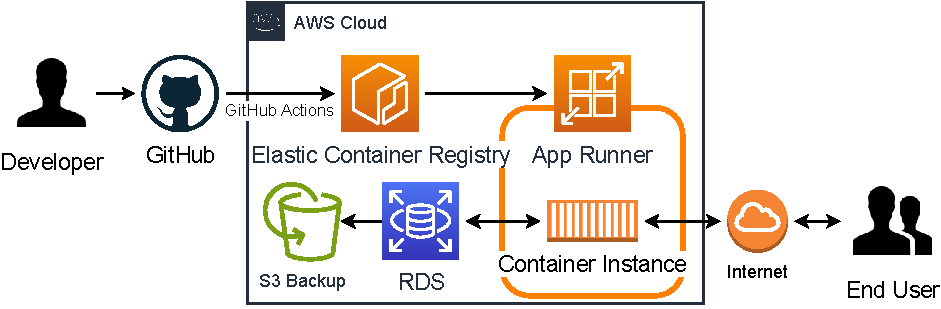
\includegraphics[width=15cm]{./images/external-design/network-design.pdf}
  \caption{ネットワーク構成図}
  \label{fig:network-design}
\end{figure}
\section{セキュリティ対策}
\subsection{ユーザー認証}
ユーザー登録の際、メールで認証用のURLを送信する。
そのURLをクリックすることで、ユーザー登録が完了する。
この手続きにより、ユーザーが本人であることを確認し、スパム登録を防ぐ。
\subsection{パスワードのハッシュ化}
パスワードは、ハッシュ化して保存する。
ハッシュ化することで、データベースの管理者であっても、パスワードを閲覧することができない。
\subsection{SQLインジェクション}
SQLインジェクションを防ぐために、SQLクエリを直接記述するのではなく、ORMを用いてSQLクエリを生成する。
\subsection{SSL通信}
SSL通信を用いることで、ユーザーが本アプリケーションにアクセスする際の通信を暗号化することができる。
\section{障害対策}
\subsection{ハードウェア障害}
AWS上にバックエンドを構築することで、AWSの障害以外では、ハードウェア障害が発生することはない。
データベースのバックアップは、Amazon S3を用いて行う。バックアップウィンドウは、深夜0時から0時30分までとし、バックアップデータは10日間保持する。
\subsection{ソフトウェア障害}
バックエンドは、Amazon Elastic Container Service上で動作するDockerコンテナである。
バックエンドのソフトウェア障害は、Dockerコンテナの再起動によって解決する。
復旧のために停止が許容される時間は、5分とする。
「落ちない」ではなく、「素早く復旧」を目標とする。
\subsection{アプリケーション開発及び、テストの障害対策}
開発者各々の環境に影響されない開発を行うためにDockerを採用した。
また、テストの際には、GitHub Actionsを用いて、自動テストを行う。

\end{document}